\documentclass[12pt, a4paper]{report}

\usepackage[czech]{babel}
\usepackage[IL2]{fontenc}
\usepackage[utf8]{inputenc}
\usepackage{lmodern}  % lepší kvalita PDF

\usepackage[a4paper,top=3cm,bottom=3cm,left=3cm,right=3cm,marginparwidth=1.75cm]{geometry}

\usepackage{amsmath}
\usepackage{graphicx}
\usepackage{titling}
\usepackage{enumitem}
\usepackage[colorlinks=true, allcolors=black]{hyperref}
\usepackage{url}
\usepackage{caption}
\usepackage{float}

\usepackage{pdfpages}

\title{Klasifikace dokumentů}
\def \thesubtitle {Semestrální práce z předmětu KIV/UIR}
\author{Patrik Harag}
\def \theauthoremail {harag@students.zcu.cz}
\def \theauthorid {(A15B0034P)}

\begin{document}

\begin{titlepage}
	\begin{figure}
		
\includegraphics[height=50mm]{img-fav-logo}
	\end{figure}
	
	\centering
	{\large \hspace{1mm} \par} % tady musí být nějaký text jinak nefunguje vertikální odsazení
	\vspace{15ex}
	
	{\scshape\Large \thesubtitle \par}
	\vspace{1.5ex}
	{\huge\bfseries \thetitle \par}
	\vspace{2ex}
	{\Large\itshape \theauthor \par}
	\vspace{2ex}
	{\texttt{\theauthoremail} \par}
	\vspace{1ex}
	{\texttt{\theauthorid} \par}
	\vspace{5ex}
	{{Celková doba řešení: \textgreater30 h} \par}
	
	\vfill

	{\large \today\par}
\end{titlepage}

% strana s obsahem
\setcounter{page}{0} 
\tableofcontents
\thispagestyle{empty}


\chapter{Zadání}
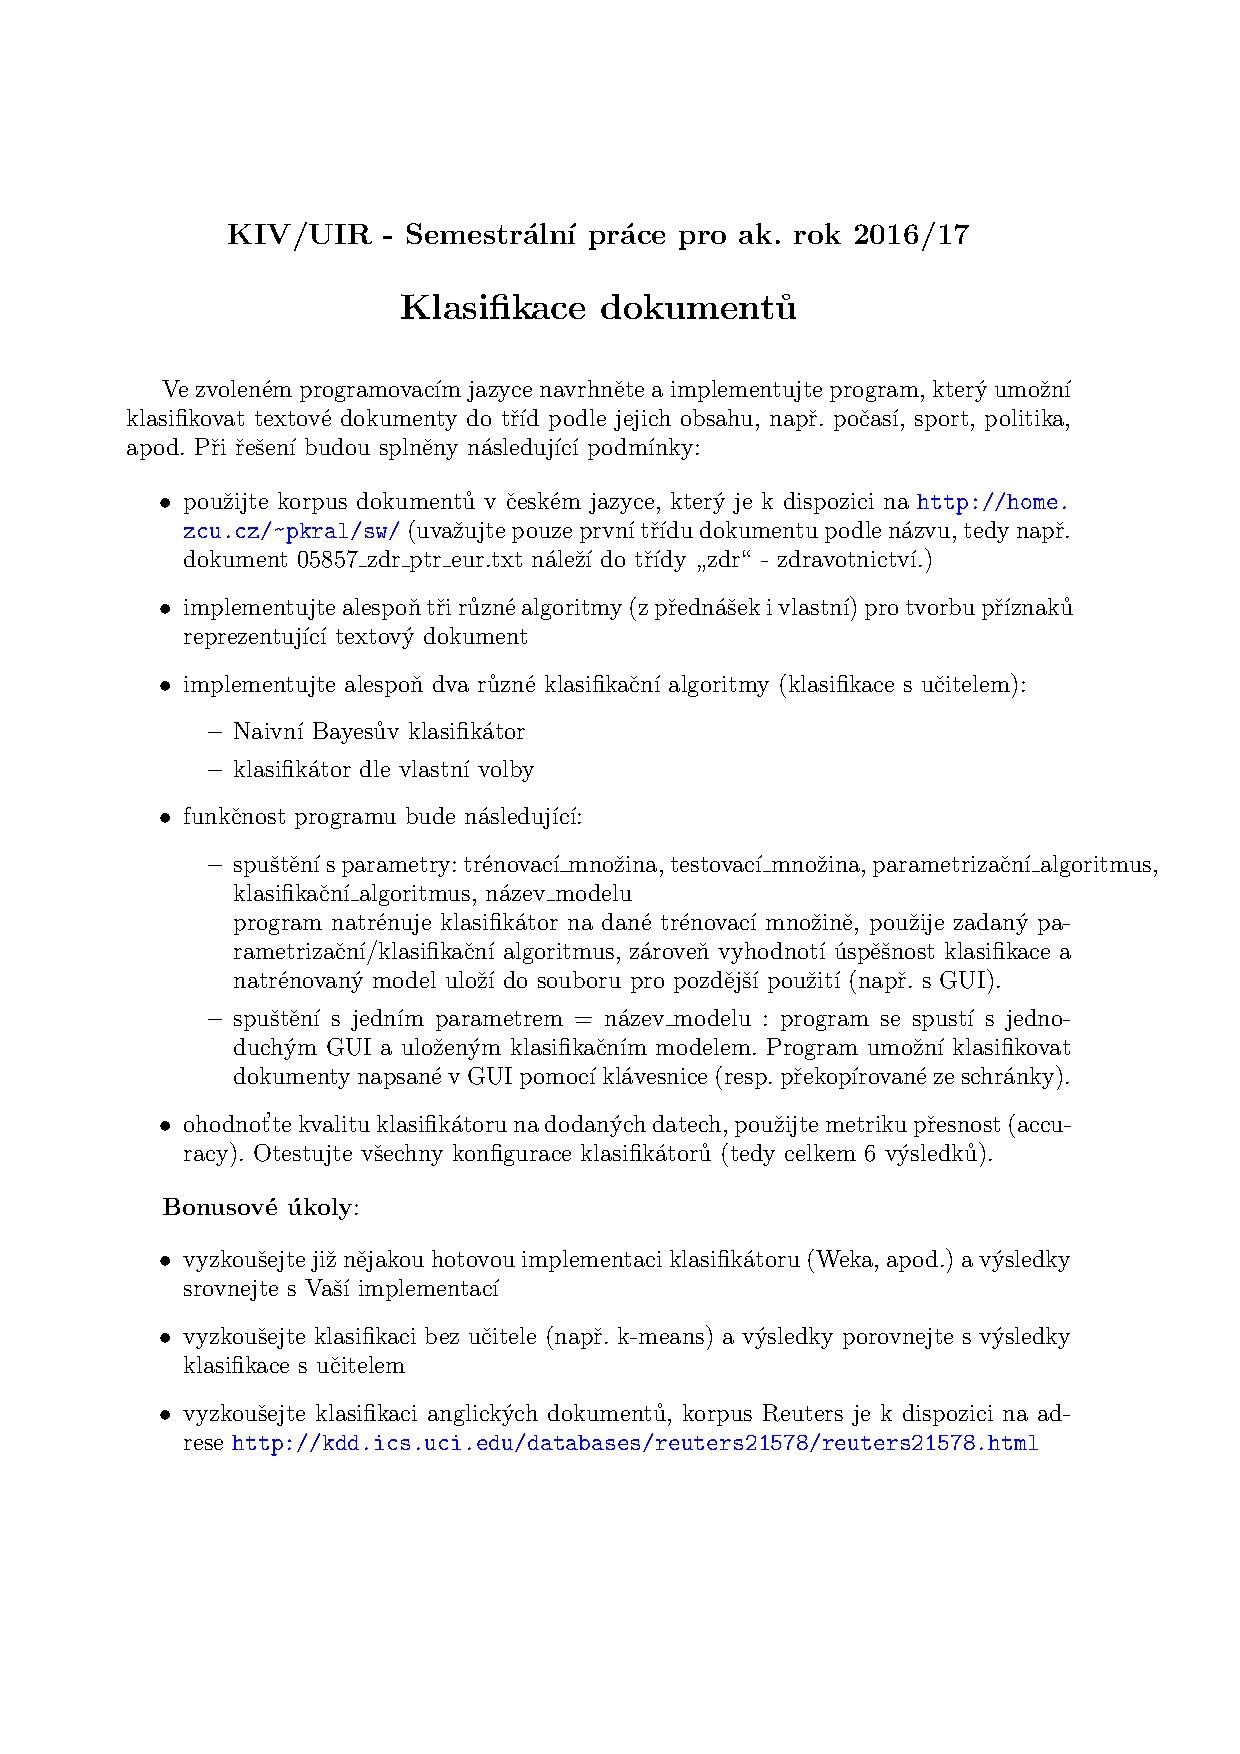
\includepdf[pages={1}]{assignment.pdf}


\chapter{Analýza}

\section{Načtení dat}
Korpus, který budeme využívat, obsahuje textové dokumenty s kódováním \mbox{\emph{UTF-8}}. Tyto texty bude nutné nejprve načíst a rozdělit na jednotlivá slova. Poté může následovat předzpracování.

\section{Předzpracování}
\label{sec:preprocessing}
Dá se očekávat, že velký vliv na výsledek klasifikace bude mít předzpracování textových dokumentů. 

\paragraph{Předzpracování může zahrnovat následující:}
\begin{itemize}
	\item Sjednocení velikosti písmen.
	\item Odstranění čísel. Případně jejich sjednocení na jedinou hodnotu, která bude mít význam \uv{nějaké číslo}.
	\item Odstranění ostatních nepísmenných znaků a sekvencí (interpunkční znaménka).
	\item Lemmatizace -- převedení slov do základního tvaru. Nejjednodušší metoda je pomocí slovníku.
	\item Odstranění slov, které nenesou žádný význam, tzv. \uv{stop words}, neboli \uv{stop slova}. V první fázi pomocí slovníku.
\end{itemize}

\paragraph{Další způsoby předzpracování aplikovatelné až po načtení všech dat:}
\begin{itemize}
	\item Odstranění slov, která se v dokumentech vyskytují pouze vzácně.
	\item Odstranění slov, která se naopak vyskytují skoro ve všech dokumentech.
\end{itemize}

\section{Výběr způsobu reprezentace dokumentů}
\label{sec:fv}
Možnosti:
\begin{itemize}
	\item Reprezentace binárním vektorem -- dokument je reprezentován jako binární vektor, ve kterém jednička znamená, že se slovo v dokumentu vyskytuje. Nevýhodou tohoto přístupu je nutnost omezit množinu slov a paměťová náročnost.
	\item Frekvenční reprezentace -- slovník, kde klíčem je slovo a hodnotou počet jeho výskytů. Může být normováno délkou článku.
	\item TF-IDF reprezentace -- jako frekvenční reprezentace, vážená TF-IDF. \cite{wiki:tfidf} Slova s větší váhou budou mít následně větší vliv při určování podobnosti vektorů.
\end{itemize}\section{Výběr klasifikátorů}

\subsection*{Naivní Bayesův klasifikátor}
Vychází z Bayesovy věty o podmíněných pravděpodobnostech a zjednodušuje ji pro případ, kdy jsou na sobě jednotlivé jevy nezávislé.

Tento klasifikátor se často používá pro klasifikaci textů, především pro svoji jednoduchost. \cite{rennie2003tackling}

\subsection*{Algoritmus k-nejbližších sousedů}
Tato metoda se ve své nejjednodušší podobě uloží celou trénovací množinu, při klasifikaci najde \emph{k} nejbližších prvků a podle nich určí třídu, do které neznámý prvek pravděpodobně patří. Přestože je tato metoda velmi jednoduchá, je možné s ní dosáhnout velmi dobrých výsledků. \cite{beyer1999nearest}

Pro výpočet vzdálenosti prvků lze použít např. euklidovská nebo Hammingova metrika.

\begin{figure}[h]
	\centering
	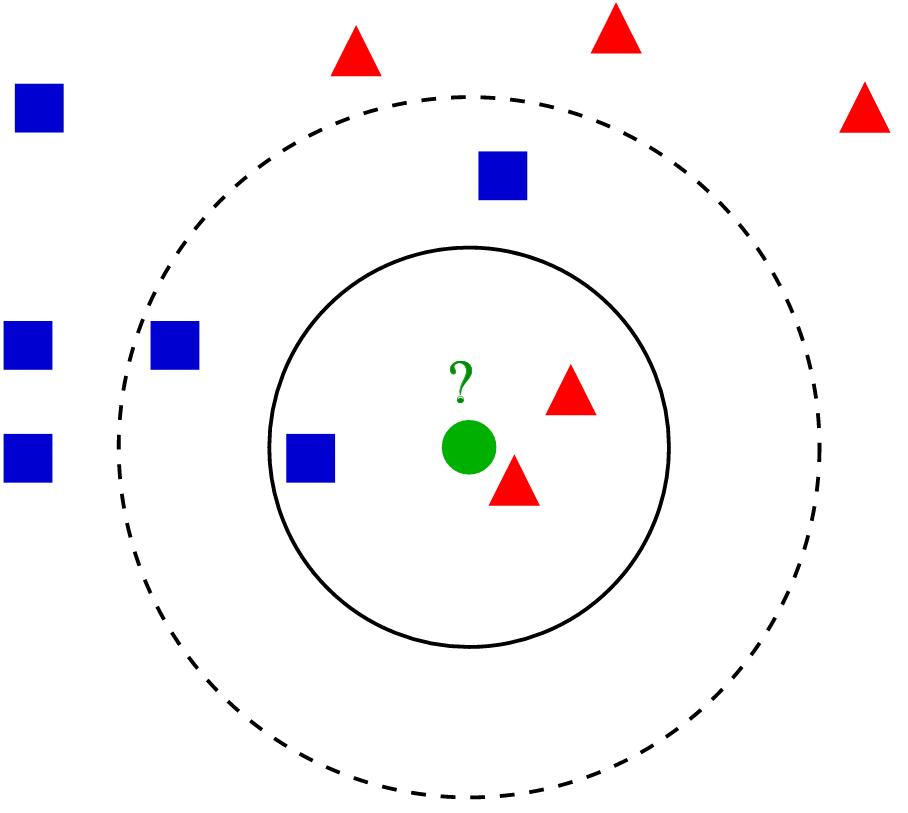
\includegraphics[width=0.3\linewidth]{img-knn}
	\caption[]{Příklad rozhodování algoritmu k-nejbližších sousedů. Pro $k=3$ bude výsledek \emph{červená} a pro $k=5$ bude výsledek klasifikace modrá. Zdroj: \cite{wiki:knn}}
\end{figure}

\chapter{Návrh řešení}
Program bude realizován v programovacím jazyce Java. Pro uživatelské rozhraní a bude použit framework JavaFX.

\paragraph{Modely} Ve zdrojovém kódu jej bude představovat rozhraní \emph{Model}. Budou implementovány všechny metody předzpracování popsané v sekci \ref{sec:preprocessing} a dále vektory příznaků v binární, \emph{frekvenční} a \emph{TF-IDF} reprezentaci, popsané v sekci \ref{sec:fv}. Oba dva způsoby budou implementovány i v redukované formě -- všechny dokumenty z jedné třídy sloučeny do jednoho dokumentu. Vzniknou tak čtyři různé způsoby reprezentace dokumentů.

\paragraph{Klasifikátory} Budou implementovány klasifikátory \emph{naivní Bayesův klasifikátor} a \emph{algoritmus k-nejbližších sousedů}. Oba tyto klasifikátory budou implementovat rozhraní \emph{Classifier} a budou přijímat \emph{Model}. Pro určení vzdálenosti dvou vektorů příznaků bude použita euklidovská vzdálenost.


\chapter{Popis řešení}

\section{Balíček cz.harag.uir.sp.app}
Obsahuje aplikační část -- vstupní třídu, která zpracovává vstup z příkazové řádky a grafické uživatelské rozhraní.

\paragraph{Třídy:}
\begin{itemize}
	\item \emph{Main} -- vstupní řída
	\item \emph{ModelProvider} -- výčtový typ dostupných modelů (parametrizačních algoritmů)
	\item \emph{ClassifierProvider} -- výčtový typ dostupných klasifikátorů
	\item \emph{App} -- třída zavádějící JavaFX aplikaci
	\item \emph{FXMLDocumentController} -- FXML kontroler (obsluha GUI)
\end{itemize}

\section{Balíček cz.harag.uir.sp.classification}
Obsahuje část zabývající se klasifikací.

\paragraph{Třídy:}
\begin{itemize}
	\item \emph{Data} -- reprezentace dokumentu po načtení (seznam slov + třída)
	\item \emph{DataLoader} -- třída načítající dokumenty
	
	\item \emph{Classifier} -- rozhraní pro klasifikátor
	\item \emph{NaiveBayesClassifier} -- naivní Bayesův klasifikátor
	\item \emph{NearestNeighbourClassifier} -- implementace metody nejbližšího souseda
	\item \emph{ClassifierIO} -- řeší ukládání a načítání klasifikátorů (pomocí serializace)
	
	\item \emph{Utils} -- obsahuje pomocné metody
\end{itemize}

\begin{figure}[h]
	\centering
	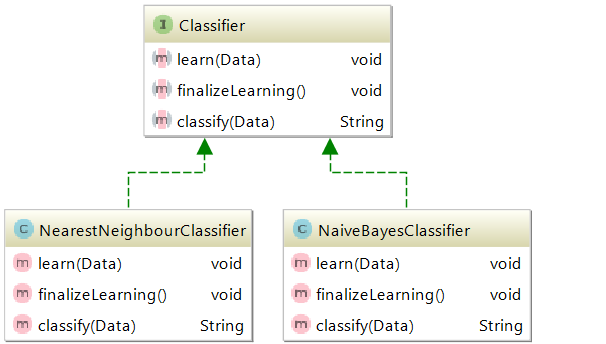
\includegraphics[width=0.8\linewidth]{img-class-h}
	\caption{Hierarchie klasifikátorů.}
	\label{fig:img-class-h}
\end{figure}

\section{Balíček cz.harag.uir.sp.classification.model}
Obsahuje třídy, které patří do modelu (kromě předzpracování).

\paragraph{Třídy:}
\begin{itemize}
	\item \emph{FeatureVector} -- rozhraní pro vektor příznaků
	\item \emph{BinVector} -- binární reprezentace dokumentu
	\item \emph{TfVector} -- frekvenční reprezentace dokumentu
	\item \emph{TfIdfVector} -- \emph{TF-IDF} reprezentace dokumentu

	\item \emph{Model} -- rozhraní pro model
	\item \emph{ModelBase} -- abstraktní třída implementující model
	\item \emph{BinVectorModel} -- model používající binární reprezentaci dokumentů
	\item \emph{BinVectorReducedModel} -- model používající redukovanou binární reprezentaci dokumentů
	\item \emph{TfVectorModel} -- model používající frekvenční reprezentaci dokumentů
	\item \emph{TfVectorReducedModel} -- model používající redukovanou frekvenční reprezentaci dokumentů
	\item \emph{TfIdfVectorModel} -- model používající \emph{TF-IDF} reprezentaci
	\item \emph{TfIdfVectorReducedModel} -- model používající redukovanou \emph{TF-IDF} reprezentaci dokumentů

	\item \emph{IdfProvider} -- rozhraní pro třídu, která vypočítá \emph{IDF} (\emph{inverse document frequency}) pro výpočet \emph{TF-IDF}
	\item \emph{IdfProviderImpl} -- implementace \emph{IdfProvider}
\end{itemize}

\begin{figure}[H]
	\centering
	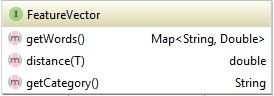
\includegraphics[]{img-fv-i}
	\caption{Rozhraní \emph{FeatureVector}.}
	\label{fig:img-fv-i}
\end{figure}

\begin{figure}[H]
	\centering
	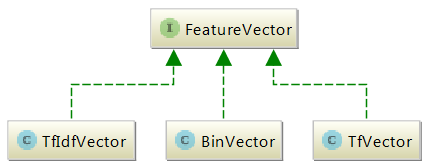
\includegraphics[width=0.35\linewidth]{img-fv-h}
	\caption{Hierarchie tříd implementujících \emph{FeatureVector}.}
	\label{fig:img-fv-h}
\end{figure}

\begin{figure}[H]
	\centering
	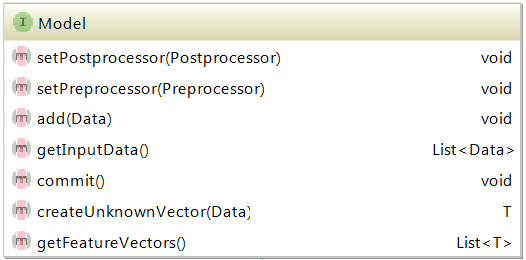
\includegraphics[width=0.7\linewidth]{img-model-i}
	\caption{Rozhraní \emph{Model}.}
	\label{fig:img-model-i}
\end{figure}

\begin{figure}[H]
	\centering
	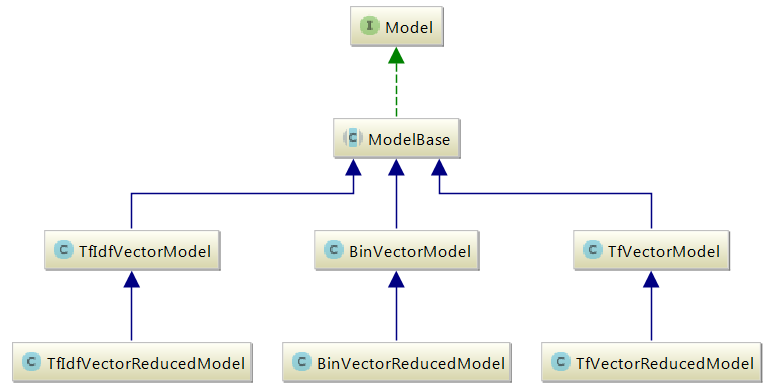
\includegraphics[width=0.7\linewidth]{img-model-h}
	\caption{Hierarchie tříd implementujících \emph{Model}.}
	\label{fig:img-model-h}
\end{figure}

\section{Balíček cz.harag.uir.sp.classification.processing}
Obsahuje třídy zabývající se předzpracováním dokumentů.

\begin{itemize}
	\item \emph{Preprocessor} -- rozhraní pro třídu která předzpracovává dokumenty. Dostává proud slov, které je možné filtrovat, modifikovat atd.
	\item \emph{Preprocessors} -- obsahuje připravené pre-procesory.
	\item \emph{StopWordsFilter} -- filtruje slova, která jsou ve slovníku.
	\item \emph{Lemmatizer} -- převádí slova do základního tvaru. Používá slovník.

	\item \emph{Postprocessor} -- rozhraní pro třídu která, podobně jako \emph{Preprocessor}, předzpracovává dokumenty. Rozdíl je v tom, že \emph{Postprocessor} je aplikován až po načtení všech dokumentů. Viz \ref{sec:preprocessing}.
	\item \emph{PostprocessorCombined} -- slouží ke skládání post-procesorů
	\item \emph{PostprocessorRemoveInEveryClass} -- Odebere slova, která jsou obsažena ve všech třídách.
	\item \emph{PostprocessorRemoveRare} -- Odebere slova, která mají počet výskytů menší než minimální počet.
\end{itemize}

\section{Digram tříd}
\begin{figure}[H]
	\centering
	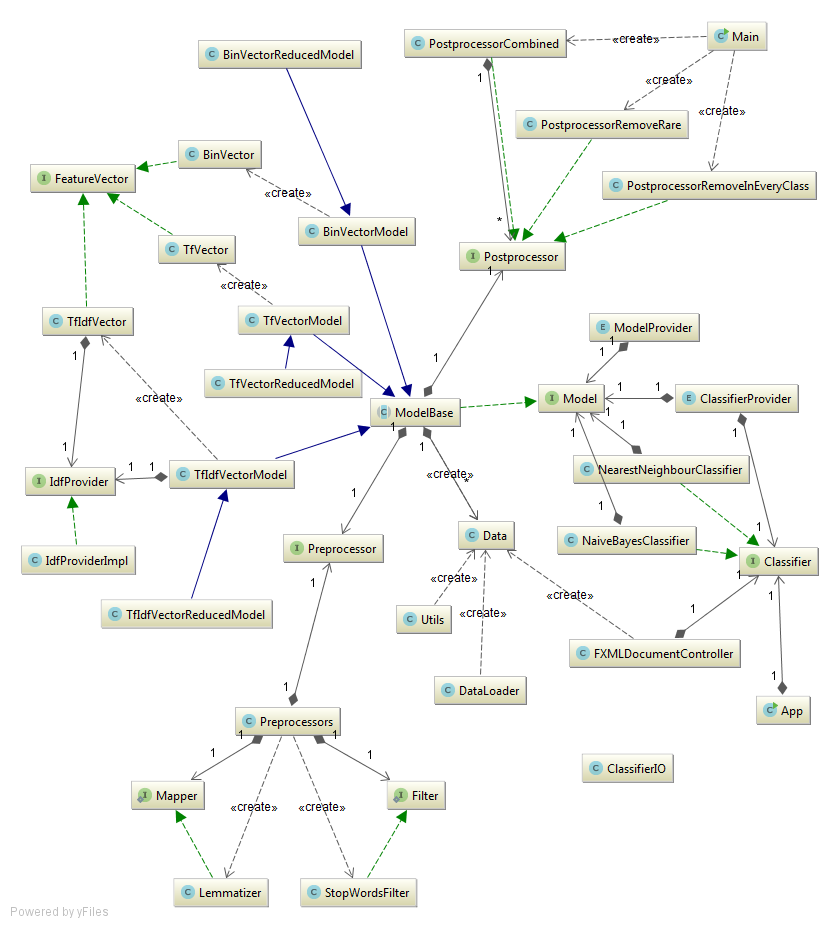
\includegraphics[width=1\linewidth]{img-uml}
	\caption{Diagram tříd.}
	\label{fig:img-uml}
\end{figure}


\chapter{Uživatelská dokumentace}
\section{Sestavení}
Pro sestavení je vyžadován nástroj Maven 3 a JDK 8.
Sestavení proběhne po zadání \emph{mvn install} do příkazové řádky v kořenovém adresáři.

\section{Spuštění}
Spuštění vyžaduje JRE 8. Program se spustí zadáním \emph{java -jar program.jar} následovaný parametry.

\subsection*{Nápověda}
Spuštění bez parametrů vypíše do konzole nápovědu.

\subsection*{Natrénování klasifikátoru}
Spuštění s parametry: \emph{trénovací\_množina}, \emph{testovací\_množina}, \emph{parametrizační\_algoritmus},
\emph{klasifikační\_algoritmus} a \emph{název\_modelu}. Vyvolá natrénování vybraného klasifikátoru na dané trénovací množině za použití vybraného parametrizačního algoritmu, zároveň vyhodnotí úspěšnost klasifikace na testovací množině a natrénovaný model uloží do souboru.

Trénovací a testovací množina je zadávána jako relativní nebo absolutní cesta ke složce, která obsahuje dokumenty ve formátu popsaném v zadání.\\

Dostupné parametrizační algoritmy: \emph{bin}, \emph{bin-r}, \emph{tf}, \emph{tf-r}, \emph{tf-idf}, \emph{tf-idf-r}

Dostupné klasifikační algoritmy: \emph{1nn}, \emph{naive-bayes}

\subsection*{Zobrazení GUI}
Spuštění s jedním parametrem, který udává \emph{název\_modelu}, zobrazí uživatelského rozhraní, které umožní klasifikovat texty napsané do textového pole.


\chapter{Závěr}

\section{Experimenty a výsledky}
Bylo provedeno měření přesnosti pro všechny konfigurace klasifikátorů a parametrizačních algoritmů.
V prvním experimentu byly pro trénování použity dokumenty 1-4000 a pro testování dokumenty 4001-5000 (výsledky viz tabulka \ref{tbl:results1}).
V druhém experimentu byly pro trénování použity dokumenty 1-10000 a pro testování dokumenty 10001-11955 (výsledky viz tabulka \ref{tbl:results2}).

\begin{table}
	\caption{Přesnost klasifikátoru při použití daného parametrizačního algoritmu.}
	\centering
	\label{tbl:results1}
	\begin{tabular}{p{.3\linewidth}|*{2}{p{.15\linewidth}}}
		Parametrizační alg. & 1nn & naive-bayes \\
		\hline
		bin & 0.31 & 0.75 \\
		bin-r & 0.06 & 0.06 \\
		tf & 0.36 & 0.75 \\
		tf-r & 0.67 & 0.06 \\
		tf-idf & 0.40 & 0.75 \\
		tf-idf-r & 0.68 & 0.06 \\
	\end{tabular}
\end{table}

\begin{table}
	\caption{Přesnost klasifikátoru při použití daného parametrizačního algoritmu.}
	\centering
	\label{tbl:results2}
	\begin{tabular}{p{.3\linewidth}|*{2}{p{.15\linewidth}}}
		Parametrizační alg. & 1nn & naive-bayes \\
		\hline
		bin & 0.4358 & 0.8281 \\
		bin-r & 0.0563 & 0.0563 \\
		tf & 0.4808 & 0.8281 \\
		tf-r & 0.7294 & 0.0563 \\
		tf-idf & 0.5315 & 0.8281 \\
		tf-idf-r & 0.6895 & 0.0563 \\
	\end{tabular}
\end{table}

\paragraph{Pozorování:}
\begin{itemize}
	\item Přesnost klasifikátorů roste s počtem trénovacích dat. Při velikosti trénovací množiny kolem 500 dokumentů byla úspěšnost klasifikace obvykle kolem 50 \%.
	\item Použití TF-IDF nemá na menších datech pozitivní vliv na přesnost klasifikace, spíše naopak. Ale zde již bylo dostatečné množství trénovacích dat, a tak došlo k vylepšení přesnosti.
	\item Parametrizační algoritmy, které využívají redukci všech dokumentů dané třídy do jediného, nefungují s naivním Bayesovým klasifikátorem. To je dáno strukturou tohoto klasifikátoru.
	\item Pro klasifikátor podle nejbližšího souseda je redukce naopak velmi výhodná -- obvykle dává lepší výsledek, za kratší čas a při nižší paměťové náročnosti.
	\item Během vývoje se u metody \emph{k}-nejbližších sousedů příliš neosvědčilo použití \emph{k} jiného než 1.
	\item Odebírání slov, které se v dokumentech vyskytují pouze jednou nemělo pozitivní vliv na úspěšnost klasifikace, proto nakonec nebylo použito (třída \emph{PostprocessorRemoveRare}).
\end{itemize}

\section{Zhodnocení}
Vytvořili jsme program pro klasifikaci dokumentů, který dává celkem uspokojivé výsledky.

Jediný potenciální problém je jeho pomalý chod některých algoritmů v případě velkého množství vstupních dat. To je však problém, který by se dal v případě nutnosti řešit. Kritické části kódu byly paralelizovány.


\bibliographystyle{plain}
\bibliography{sources}

\end{document}